
\section{Harmonic parametrisation of the Fermi surface}
    \label{Sec:ResD:TightBindingFits}

An analytic form for the Fermi surface can be obtained using a harmonic expansion of sin and cosine functions as described by Bergemann \etal~\cite{Bergemann2000}. Primarily this was done so as to provide a convenient way to reconstruct the Fermi surface without necessitating \ac{DFT} calculations for future use in models. The expansion is as described as,
\begin{equation}
\label{Eqn:ResD:HarmonicExpansion}
k_F(\phi, \kappa) = \sum_{\substack{\mu,\nu \geq 0 \\ \mu \textrm{even}}}
    k_{\mu\nu}\cos\nu\kappa 
    \begin{cases}
        \cos{\mu\phi} \hspace{8pt} &(\mu\hspace{-6pt}\mod4 = 0) \\
        \sin{\mu\phi} \hspace{8pt} &(\mu\hspace{-6pt}\mod4 = 2)
    \end{cases}
\end{equation}
where $k_F$ is the Fermi surface in k-space, $\kappa = ck_z/2$, $c$ is the unit cell height and $\phi$ is the polar angle. A slightly different set of functions would be necessary to fit the electron Fermi surface in the adjacent corners due to the screw symmetry, however only one electron sheet was fitted.

The two dimensional fits were performed using a least square fitting routine using MATLAB on the \ac{DFT} data shifted as described in the previous section. The number of terms for the fits were increased until the residuals ceased to change appreciably. Fit parameters are presented in table~\ref{Tab:ResD:HarmonicParams}. Due to the skewed nature of the $k_z$ dispersion of the outer hole surface $20$ terms were necessary to obtain a reasonable fit to the corrected \ac{DFT} data however electron surfaces could be fitted well with $9$ terms and the inner hole surface with $10$ terms.  The final analytical function was then used to create an `energy dispersion' on a discrete grid of $k$-points such that plotting an isosurface at $\epsilon = \unit{0}{\textrm{Ry}}$ correctly recreated the Fermi surface\footnote{The resulting dispersion was not physical and simply served as a computational structure to pass the shape of the Fermi surface to the MATLAB code, energy values at $k$-point away from the Fermi surface are somewhat arbitrary.}. Using this dispersion in the existing MATLAB code, extremal orbits were then calculated as a check of how well it matches the original data. The results of this are presented in figure~\ref{Fig:ResD:TightBindingFitRotationPlot}. As you can see, although the fits were to the modified \ac{DFT} calculations, the fits are also reasonably accurate at modelling the measured data.
\begin{figure}[htbp]
    \begin{center}
        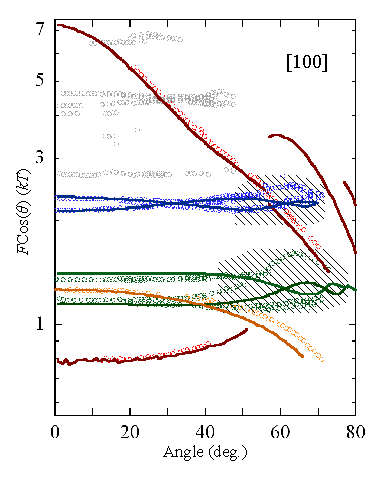
\includegraphics[scale=0.9]{Chapter-dHvABaFe2P2/Figures/AngleDepMeasurements/TightBindingFits/TightBindingFits}
        \caption{Rotation plots for the harmonic fits calculated from the c-axis down towards $[100]$.}
        \label{Fig:ResD:TightBindingFitRotationPlot}
    \end{center}
\end{figure}
\begin{table}
    \caption{Harmonic expansion fit parameters performed on the shifted \ac{DFT} Fermi surfaces.}
    \label{Tab:ResD:HarmonicParams}
    \begin{center}
{\small
    \begin{tabular}[htbp]{lrrrr}
\toprule
Factor	& $\alpha$	& $\beta$	& $\gamma$	& $\delta$	\\
\midrule
$k_{00}$	&  1.90796e$^{-1}$	&  2.59538e$^{-1}$	&  2.58282e$^{-1}$	&  1.35031e$^{-1}$	\\
$k_{02}$	& -1.32049e$^{-2}$	& -1.01956e$^{-3}$	&  0		& 0		\\
$k_{04}$	&  9.24279e$^{-4}$	&  4.28603e$^{-4}$	& -1.01085e$^{-2}$	&  1.95065e$^{-3}$	\\
$k_{20}$	&  4.30196e$^{-4}$	& -1.51226e$^{-4}$	& -1.46090e$^{-1}$	& -6.75502e$^{-2}$	\\
$k_{22}$	&  3.23365e$^{-4}$	&  1.91896e$^{-4}$	&  0		& 0		\\
$k_{24}$	& -9.30815e$^{-2}$	& -4.23320e$^{-2}$	&  1.13859e$^{-2}$	& -5.31077e$^{-3}$	\\
$k_{40}$	& -1.64499e$^{-2}$	&  5.02893e$^{-3}$	&  6.15148e$^{-2}$	& -5.70262e$^{-3}$	\\
$k_{42}$	& -1.49159e$^{-2}$	& -7.07858e$^{-3}$	&  0		& 0		\\
$k_{44}$	& -6.14076e$^{-4}$	& -2.86767e$^{-4}$	& -9.49526e$^{-3}$	&  5.28982e$^{-3}$	\\
$k_{60}$	& 0		& 0		& -1.85170e$^{-2}$	& -1.22242e$^{-3}$	\\
$k_{64}$	& 0		& 0		& -9.04247e$^{-4}$	& -2.82851e$^{-4}$	\\
$k_{80}$	& 0		& 0		& -6.79607e$^{-3}$	& -2.22767e$^{-3}$	\\
$k_{84}$	& 0		& 0		&  1.61746e$^{-3}$	& -1.90500e$^{-3}$	\\
$k_{100}$	& 0		& 0		&  1.07007e$^{-2}$	& 0		\\
$k_{104}$	& 0		& 0		&  7.97948e$^{-4}$	& 0		\\
$k_{120}$	& 0		& 0		& -3.89161e$^{-3}$	& 0		\\
$k_{124}$	& 0		& 0		& -1.57292e$^{-3}$	& 0		\\
$k_{140}$	& 0		& 0		& -1.81052e$^{-3}$	& 0		\\
$k_{144}$	& 0		& 0		&  3.81207e$^{-4}$	& 0		\\
$k_{160}$	& 0		& 0		&  3.04268e$^{-3}$	& 0		\\
$k_{164}$	& 0		& 0		&  1.14420e$^{-3}$	& 0		\\
$k_{180}$	& 0		& 0		& -1.07753e$^{-3}$	& 0		\\
$k_{184}$	& 0		& 0		& -4.92181e$^{-4}$	& 0		\\
\bottomrule
    \end{tabular}
}
    \end{center}
\end{table}

% Band 4
% nu_cos_vals = [0 2 4];
% mu_cos_vals = [0 4];
% mu_sin_vals = [2];
% BAND_NUM = 4;
% OUT_FILENAME = 'band4_pseudo_fs.mat';
% P = [0.190795650551417;-0.0132049241203695;0.000924278555081638;0.000430196076110210;0.000323365284403928;-0.0930815369372282;-0.0164499250846804;-0.0149158554339246;-0.000614076088937712];

% Band 3
% nu_cos_vals = [0 2 4];
% mu_cos_vals = [0 4];
% mu_sin_vals = [2];
% BAND_NUM = 3;
% OUT_FILENAME = 'band3_pseudo_fs.mat';
% P = [0.259537885523148;-0.00101956346539010;0.000428602835795347;-0.000151225676919844;0.000191895525922163;-0.0423319597296428;0.00502893573615497;-0.00707857925603053;-0.000286767052816500];

% Band 2
% nu_cos_vals = [0 2 4 6 8 10 12 14 16 18];
% mu_cos_vals = [0 4];
% mu_sin_vals = [];
% BAND_NUM = 2;
% OUT_FILENAME = 'band2_pseudo_fs.mat';
% P = [0.258282295891213;-0.0101085190499327;-0.146089742845922;0.0113858941052011;0.0615148335223954;-0.00949526005728540;-0.0185169711239324;-0.000904247435640945;-0.00679607129328513;0.00161745790960140;0.0107007232759639;0.000797948298873890;-0.00389161131091256;-0.00157292133954998;-0.00180519311058468;0.000381207138913101;0.00304267547098585;0.00114419875689493;-0.00107753360762167;-0.000492181334709838];

% Band 1 
% nu_cos_vals = [0 2 4 6 8];
% mu_cos_vals = [0 4];
% mu_sin_vals = [];
% P = [0.135031574336540;0.00195065231744799;-0.0675502357038337;-0.00531077032608857;-0.00570262272420267;0.00528982052397907;-0.00122242158640231;-0.000282850535526285;-0.00227673928224173;-0.00190499796892254]

